\documentclass[12pt,a4paper]{scrartcl}
\usepackage[utf8]{inputenc}
\usepackage[english]{babel}
\bibliographystyle{unsrt}
\usepackage{amsmath}
\usepackage{amsfonts}
\usepackage{amssymb}
\usepackage{graphicx}
\usepackage{enumitem}
\usepackage{rotating}

\linespread{1.2}
\begin{document}
	\title{\vspace{-4ex}Predicting network load with machine learning for VNF placement}
	\subtitle{Proposal for a master's thesis}
	\author{Christoph Kaiser \\
		kaiserc1@mail.uni-paderborn.de\vspace{1ex}}
	\maketitle
	
	\textbf{\textit{Abstract} - A problem with current algorithms for placing VNFs in a network and scaling the services is that they can typically only react to arriving requests. Replacing this reactive nature with prediction capabilities could yield results for compensating startup times, shutting down services earlier and keep services running. Also, the algorithm can scale the service proactively. Developing a machine learning model that can reliably predict new requests and what services will be called by these requests is the goal of this master thesis. A big challenge of this thesis will be the modelling of the available information as an input for neural networks. The second big task will be the modelling and training of the machine learning models.}
	
	\section{Introduction}
	Networks with Virtual Network Functions (VNF) are a heavily researched topic.
	The process of Network function virtualization creates these VNFs; here, services are build that are made up of different functions to fulfill a specific task; for example, video streaming.
	These VNFs save resources and make a network more robust to changing network load situations because each function can be placed at each physical node in a network.
	However, one of the research subjects is the scaling of the system and where to place these VNFs efficiently.
	The goal of this master thesis is to predict the network traffic that requires the algorithm to scale the network and place new VNFs.
	
	A problem with VNFs is that they take some time to start.
	As noted by \cite[p.108-109]{Mijumbi}:
	\begin{quote}
		"As can be noted, even for a single VM, the time needed for boot and basic provisioning is in the order of tens of seconds. This time grows very quickly if a higher number of VMs is required."
	\end{quote}
	When a system can only react to a request and not predict it, and the system has not yet started the VNF, the time for starting the necessary software will be added to the waiting time of the request.
	A request in this context is meant to be a request for a specific service, and all further mentions of request mean the same thing.
	The naive approach would be to have all services running on all nodes.
	However, that would defeat the purpose of function virtualization.
	Furthermore, if all services are always running at each node, it is a waste of resources, and the fulfillment of a request probably takes extra time since the VNFs take resource from each other.
	The better approach would be to predict the requests so that the system can start the service early to compensate for its startup time.
	
	A problem with algorithms like \cite{draxlerScaling} is the fact that they can only react to a request that already arrived.
	When a service request arrives for a service that was not previously started by the system, the request must wait the extra startup time in addition to the actual processing of the request.
	The same problem arises when the network has to be scaled to match the incoming requests.
	If the algorithm determines that the system needs to add a new VNF to the network, it can only do so after the request arrived.
	
	The idea of this master thesis is to rectify the problems of the reactive nature of these algorithms.
	For this purpose, the goal is to develop and test a machine learning model that can reliably predict new requests and what services the requests need.
	With these predictions, an algorithm could then compensate for the startup time of services, shut down services earlier if no new request is arriving or keep services running if a new request is imminent to arrive.
	The same is true for the scaling of the services.
	
	As mentioned earlier, the topic of VNFs is a highly researched topic.
	Also, the topic of predicting network traffic to place and scale services proactively is an even newer topic of research.
	For predicting network traffic, there are already a lot of papers, one example \cite{networkStudies}.
	There also exist many examples for traffic prediction for VNF placement and scaling; only three examples include \cite{8486320}, \cite{10.1007/978-3-319-70087-8_90} and \cite{7502957}.
	All these papers provide best practices and mistakes that can be avoided.
	
	\section{Gathering Data}
	The first major topic for this master thesis is the search for datasets used for training and testing the models.
	There are multiple sets of data available; two examples are \cite{GoogleData} and \cite{FacebookData} from google and facebook.
	These datasets contain traces from their networks.
	There are also many more sets of traces available, containing different kind of pieces of information from other networks.
	
	The first big step will be to download multiple datasets and sort through them to find the most suitable.
	What information precisely the datasets should contain will become more evident during the building of the machine learning models.
	Ideally, the data should contain the service chain that is associated with the request, but there is probably no data with service chains available since NFV (Network Function Virtualization) is not yet used in the real world.
	However, since a service chain is needed, the data needs to be annotated with an artificial service chain.
	Finding an Algorithm for creating and annotating realistic service chains will also be part of the data preparation step.
	
	The structure of the network where the traces come from could also present as a problem.
	Just from the traces, it is not possible to reconstruct the network.
	If the traces contained the routing information of the packets, it would be a possibility to reconstruct the network, but even then it would not be a guarantee.
	If the information of the network structure is even needed will become more evident in the next steps during the model building, training and testing.
	When it becomes clear that the models need the structure for accurate predictions, an artificial network structure has to be created, just like the service chain.
	
	The preparation of the data will be done using R or Python libraries since the amount of data is so high that specialized data processing libraries are needed.
	
	Another approach would be to generate Traces; this would eliminate the problem of reconstructing the network and having to modify the data.
	However, the development of a suitable algorithm to generate realistic traces would also take a high amount of time.
	It is not clear if time would be saved, trying to generate data opposed to modifying already existing data.
	Furthermore, using real data increases the credibility of the results of this master thesis.
	
	\section{Model Building}
	The central part of the thesis is the building of the machine learning models.
	To build a machine learning model, multiple libraries exist to abstract the task of creating these models.
	One of the better-known ones is Tensorflow. Google makes Tensorflow, and it is used to create machine learning models like neural networks.
	It will be the first library that will be looked at because there exist a large number of tutorials for it and in the Computer cluster of the University of Paderborn exists hardware support for Tensorflow.
	However, another library I will look at is Keras.
	Keras uses Tensorflow to build and train Neural Networks and maybe there exist advantages to use the library directly instead of more abstract Keras.
	A short time will also be spent looking at other libraries, but Tensorflow and Keras are the top two choices.
	
	After the step of choosing the library, the next task is to implement the machine learning models.
	However, the question is what kind of model should be used.
	A promising candidate is LSTM.
	LSTM, developed in 1995 \cite{lstmOrig}, stands for Long short-term memory.
	This machine learning model is a neural network, but the weight of each neuron is calculated differently than in the standard neural network.
	The essential part of LSTMs is that each neuron considers its previous values.
	In a sense, it "remembers" what it did before.
	An LSTM has what regular neural networks are missing; it has a context for what came before its current configuration. 
	
	To have a comparison for the more advanced LSTM, a basic Neural Network will also be implemented and tested how well it can predict future requests.
	Since the Neural network does not consider previous values, it will probably have deficits while predicting too far into the future.
	
	To have a baseline for the quality of the predictions from the machine learning models, an already established model will also be used.
	This model is the ARIMA model (Autoregressive integrated moving average).
	ARIMA is not used for machine learning but is a strictly statistical model.
	There exist scientific works on how ARIMA can be used to predict network traffic, only one example \cite{ArimaTraffic}. So implementing the ARIMA model should be no problem, since there exist many references.
	
	A big part of building the machine learning models is the modelling of the inputs.
	This is one of the most challenging parts, since there no standard ways of modelling the input data.
	Each model needs a new way of modelling the data, so a considerable amount of time will be needed to find efficient ways of modelling the data.
	The most challenging part here will be modelling the current network structure.
	Typically inputs for a neural network are floating point numbers ranging from 0 to 1.
	Efficiently mapping a network structure to these inputs is no trivial task.
	The problem of how to model the inputs also exists for the other attributes like the source-address, destination-address, service chain, time of request and many more possible inputs.
	However, the problem is more severe for the network structure because most attributes can not grow indefinitely. An IP-Address (V4) for example, always has a length of 32 bits.
	
	However, while modelling the inputs, the size of the network is a relevant factor.
	Theoretical there are no limits to the size of the network but finding a way of modelling the network structure, and other attributes to match a network that can scale to an indefinite size is not possible.
	So the result of the master thesis, if the structure of the network is used, will probably include a restriction on the size of the network.
	
	Also, for each kind of output, a new model is needed.
	The prediction of the load at a point in time needs one model, but predicting the load over a period of time needs an entirely different model.
	
	How these models will perform exactly is not easy to predict. However, there already exist studies on the topic of using statistical models and machine learning to predict network traffic \cite{networkStudies}.
	So before starting the model building phase information can be gathered on what to expect and what mistakes to avoid.
	
	\section{Training}
	After building the machine learning models, they will train with the data.
	The approach for training neural nets used most often is splitting of the test data into three sets.
	One set is then used to train the model; one is used to validate the training step and the last is used to test the quality of the predictions.
	Exactly how much of the data is sufficient for good predictions has many dependencies so that no assumption can be made now.
	This will get clear in the training step.
	
	It is possible that the static training and testing do not deliver the wished results for the application of predicting changing network load.
	If that is the case, training during runtime might deliver a better result.
	Instead of relying on the pre-runtime training, each new request is used during runtime to train the model continuously.
	
	\section{Evaluation}
	When the testing of the machine learning and ARIMA models is complete, the next step is comparing the test data.
	The test will have produced a large number of results.
	These results will be evaluated using R or Python.
	The comparison will include many different evaluations.
	Examples are: comparing the accuracy of prediction in the next timestep, how well the models predict going further into the future, how well the predictions work when predicting the load over a period of time instead of a point in time. How and what is evaluated must be chosen with care as it will fundamentally influence what conclusions will be the result of this thesis.
	
	The goal of this thesis is the ability to provide algorithms with predictions so that they can proactively scale the services and place VNFs in the network.
	The desired result would be a machine learning model that can predict new requests reliably.
	To fulfil the goal of this thesis, the predictions should go so far into the future that the starting time of a VNF will not interfere with fulfilling a request.
	Also, the ideal model would have predictions for all services in the output data.
	That would lead to the effect that it only takes one computation to know what services need to be started or scaled and not one computation per service, saving significant amounts of time.
	
	One more important result is how long the computation of the predictions takes.
	If the time for the computation takes longer than the time it tries to predict into the future; the result will already be outdated.
	For example, if the result should show the load in 5s and the calculation takes longer than 5s, the result will be useless.
	The ideal outcome here would be that the calculation takes only so much time that a VNF can still start. Using the example of predicting 5s into the future again, if the VNF takes 3s to start, the calculation should not take longer than 2s, so that it will not interfere with the processing.
	
	\pagebreak
	\section{Structure of the thesis and timetable}
	\begin{enumerate}[label*=\arabic*.]
		\item Introduction
		\item Related work \& Fundamentals
		\item Gathering Data
		\begin{enumerate}[label*=\arabic*.]
			\item Download and analyze
			\item Preparing the data
		\end{enumerate}
		\item Model Building
		\begin{enumerate}[label*=\arabic*.]
			\item Choosing a library
			\item Modeling the input data
			\item Building the models
		\end{enumerate}
		\item Training and testing
		\begin{enumerate}[label*=\arabic*.]
			\item Training the models
			\item Evaluating test data
		\end{enumerate}
	\end{enumerate}
	
	\begin{sidewaysfigure}
		\centering
		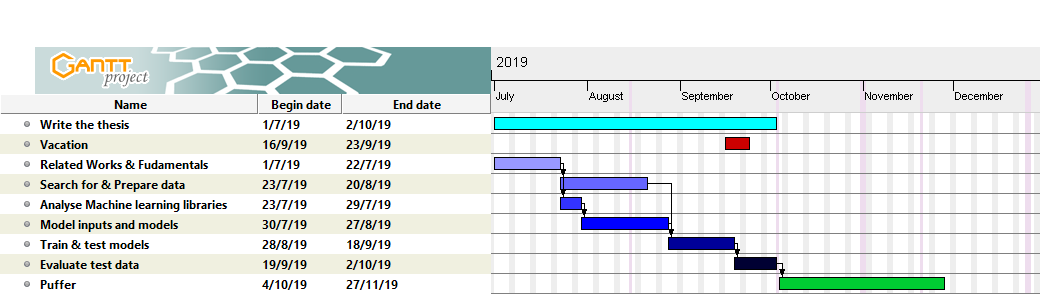
\includegraphics[width=1.0\linewidth]{Timetable/Timetable}
		\caption{Timetable}
		\label{fig:timetable}
	\end{sidewaysfigure}
	\pagebreak
	\bibliography{proposalBib}
	
	
\end{document}